\tikzstyle{end} = [circle, minimum size = 0.1cm, draw, inner sep = 0.1pt]
\tikzstyle{leaf} = [circle, minimum size = 0.6cm, draw, inner sep = 0.1pt, blue]
            
\tikzstyle{level 1}=[level distance = 1.5cm, sibling distance = 1.5cm]
\tikzstyle{level 2}=[level distance = 1.5cm, sibling distance = 3cm]
\tikzstyle{level 3}=[level distance = 1.2cm, sibling distance = 1.8cm]
\tikzstyle{level 4}=[level distance = 2cm, sibling distance = 1.3cm]


    
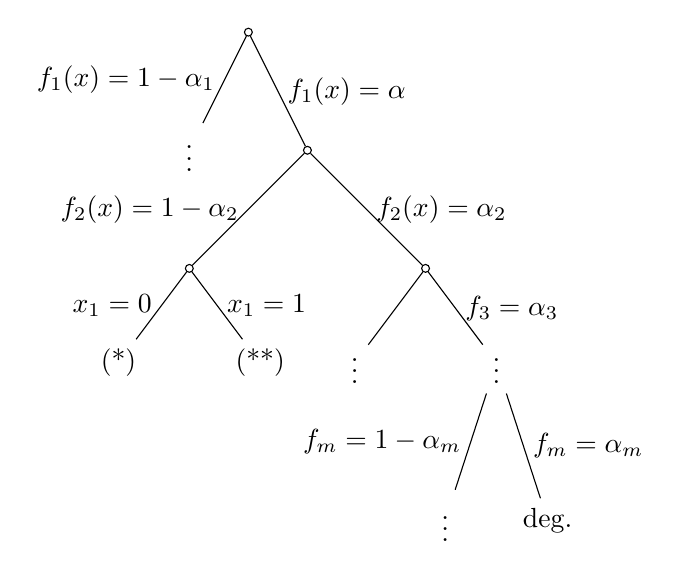
\begin{tikzpicture}[label distance = 8mm]
	\node [end] {}
	    child {
        	node {$\vdots$}
           	edge from parent
            node[left] {$f_1(x) = 1 - \alpha_1$}
        }
        child {
        	node[end] {}
            child {
		        node[end] {}
                child {
        			node {\alert{(*)}}
		           	edge from parent
        		    node[left] {$x_1 = 0$}
		        }
                child {
                  	node {\alert{(**)}}
                    edge from parent
                    node[right] {$x_1 = 1$}
                }
	            edge from parent
		        node[left] {$f_2(x) = 1 - \alpha_2$}
			}
		    child {
		        node[end] {}
                child {
        			node {$\vdots$}
		           	edge from parent
        		    node[left] {}
		        }
                child {
                  	node {$\vdots$}
                    child{
  		                node {$\vdots$}
			           	edge from parent
        			    node[left] {$f_m = 1 - \alpha_m$}
                    }
                    child{
  		                node {\alert{deg.}}
			           	edge from parent
        			    node[right] {$f_m = \alpha_m$}
                    }
                    edge from parent
                    node[right] {$f_3 = \alpha_3$}
                }
	            edge from parent
		        node[right] {$f_2(x) = \alpha_2$}
            }
           	edge from parent
            node[right] {$f_1(x) = \alpha$}
        };
\end{tikzpicture}

%%% Local Variables: 
%%% mode: latex
%%% TeX-master: t
%%% End: 
